\Chapter{}
\chapter{CRONOGRAMA DE ACTIVIDADES}
    \begin{figure}[H] 
        \caption{\doublespacing \\ \textit{Cronograma de actividades para la investigación.}} 
        \centering
        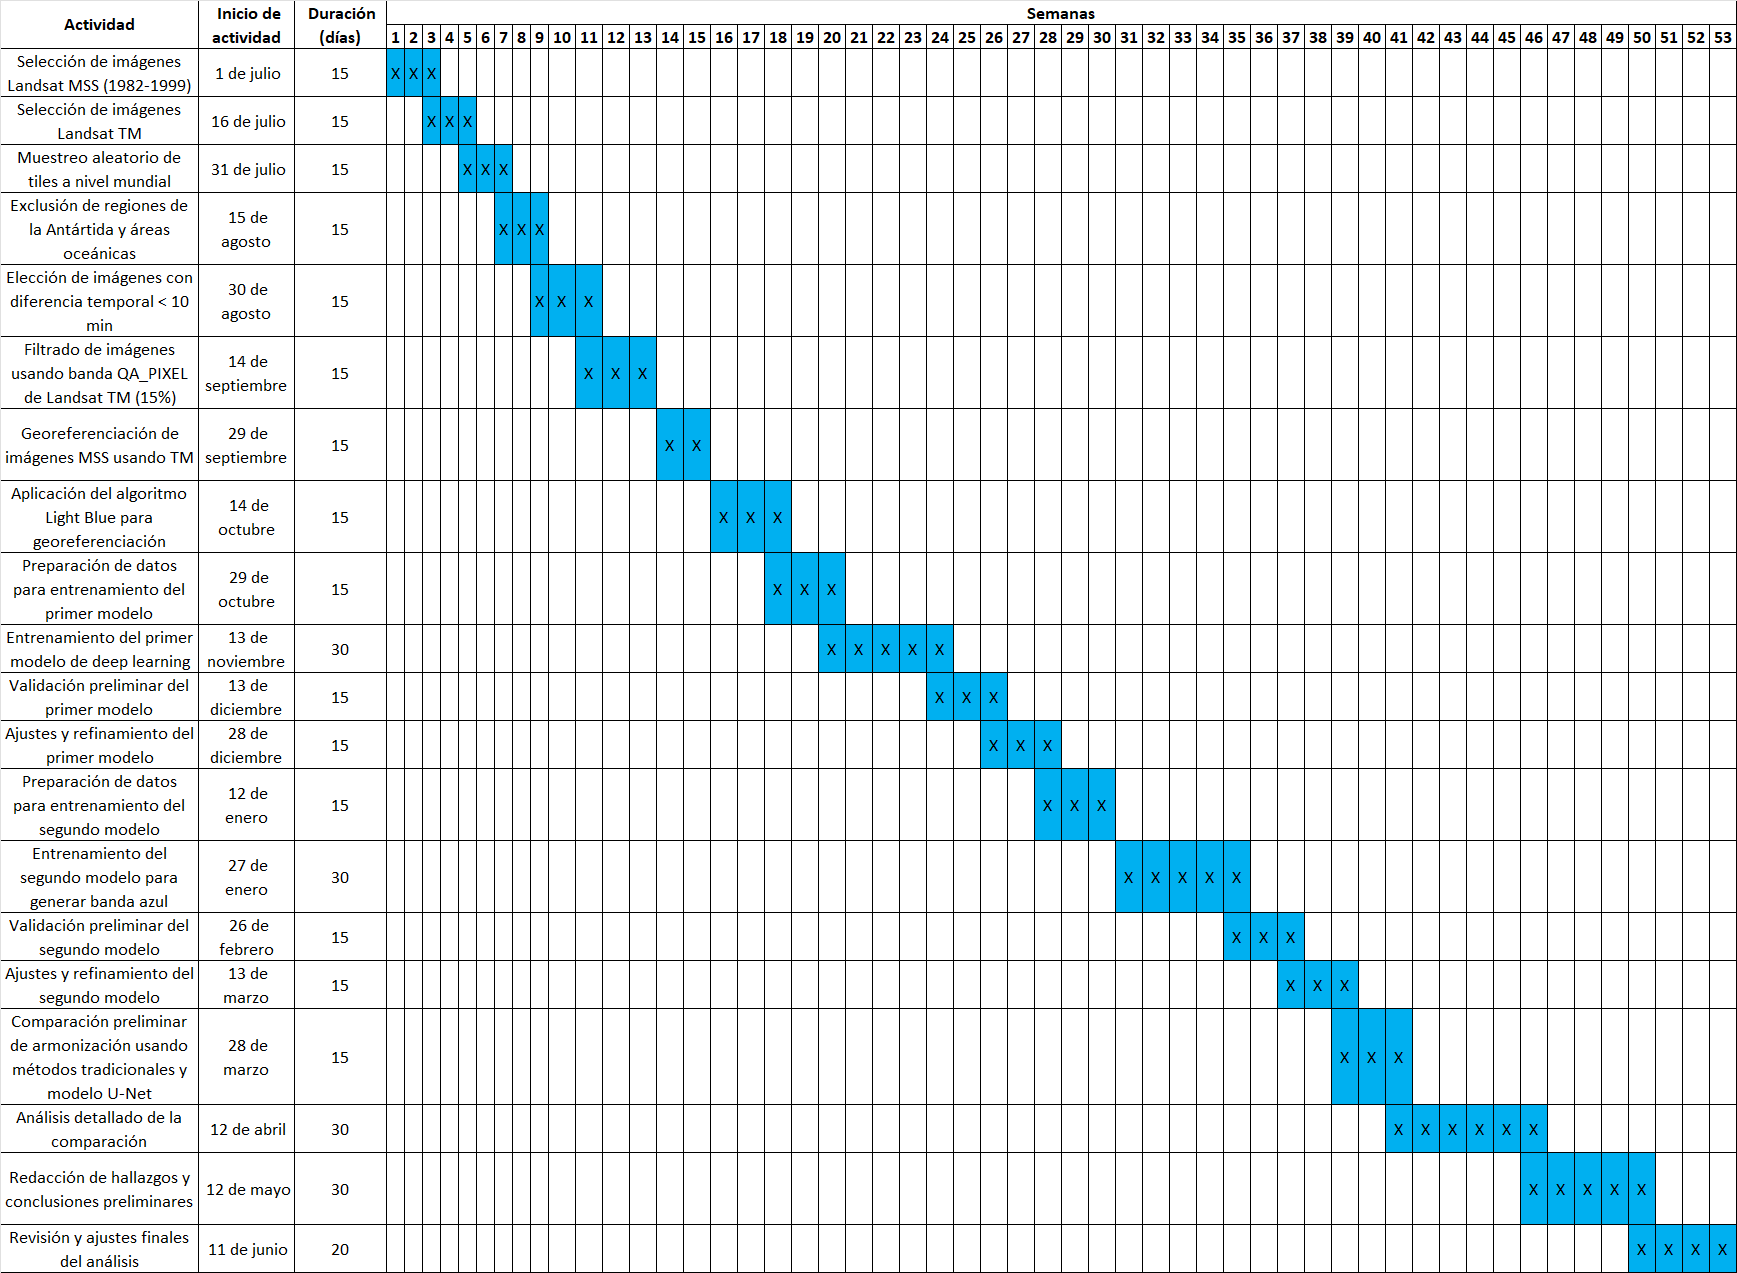
\includegraphics[width=1.12\linewidth, angle=90]{2_CAPITULO0/IMG/cronograma.png}
        \begin{justify}
            \textit{Nota.} El cronograma anual detalla la secuencia de actividades, desde la elección de imágenes Landsat hasta las modificaciones finales, organizadas semanalmente a lo largo de un año.
        \end{justify}                    
        \label{cronograma}
    \end{figure}